\section{Durchführung}
\label{sec:Durchführung}

Für den Versuch wird der in \autoref{fig:messapp} dargestellte Aufbau verwendet, wobei der He-Ne-Laser nicht um die Strahlachse schwenkbar war.

\begin{figure}[H]
	\centering
	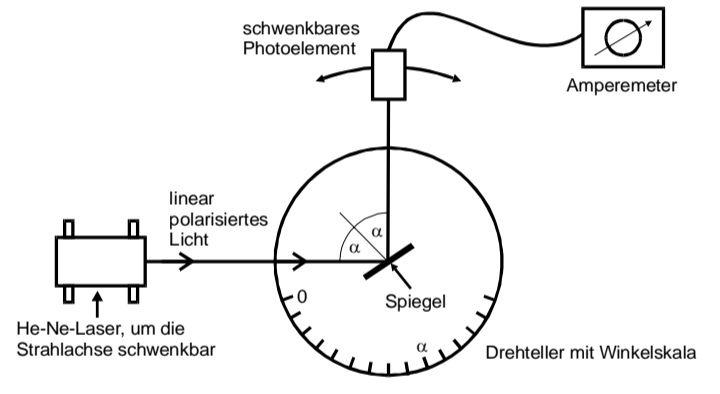
\includegraphics[width=0.6\linewidth]{data/v407Messapparatur.jpg}
	\caption{Schematische Darstellung der verwendeten Messapparatur.\cite{Anleitung407}}
	\label{fig:messapp}
\end{figure}

\noindent
Bevor die eigentliche Messung beginnen kann, muss zunächst die Messapparatur justiert werden.
Es wird hierfür der Silizium-Spiegel entfernt und eine Messung der Intensität des Laser-Strahles durchgeführt. Anschließend wird der Spiegel erneut auf dem Probehalter montiert
und so ausgerichtet, dass der Laser-Strahl dierekt auf den Laserkopf zurück reflektiert wird. Auch wird darauf geachtet, dass das Goniometer in dieser Stellung genau einen Winkel
von 0° zeigt, um später die Abweichung des Winkels zu dieser Stellung abzulesen. Anschließend ist die Justierung abgeschlosssen und die Mesung kann beginnen.
\newline\newline
Für die eigentliche Messung wird zunächst ein Winkel für die Polarisation eingestellt. Es wurden zwei Messreihen mit einem Polarisationswinkel von 0° und 90° durchgeführt.
Im Anschluss wird die Intensität des reflektierten Laserstrahles für unterschiedliche Eintrittswinkel des Lasers auf den Silizium-Spiegel gemessen. Es werden dabei Winkel in
einem Intervall von 10° bis 88° gemessen, da für Winkel unter 10° und über 88° die Messapparatur den Laser blockiert. Die Messwerte werden dabei jeweils in einem Abstand
von 2° aufgenommen.